

\chapter{Conceptual Model for Reactive Information Systems and their Services}
The challenges and opportunities arising with the growth of the Web in terms of volume and complexity inspired our research towards the reactive Web.
Therefore our starting point was the studies of related work in the context of reactivity on the Web, event composition and programmability of the Web.
In the last chapter, we pointed out how they received a lot of attention and provide powerful tools to orchestrate the rapidly growing Web.
By combining existing research in these fields we developed a conceptual model, which allows to impose smart reactivity to any \textrm{\gls{infospace}}, not only the Web.
Even though our initial set of \textrm{\glspl{infospace}} was thought to consist of \textrm{\glspl{webresource}}, our model is applicable to any \textrm{\gls{infosystem}} whose \textrm{\gls{infospace}} can be accessed and altered over interfaces, i.e. services.
Thus we introduce our conceptual model for reactive \textrm{\glspl{infosystem}} and their services in this chapter.

\begin{figure}[!ht]
  \centering
  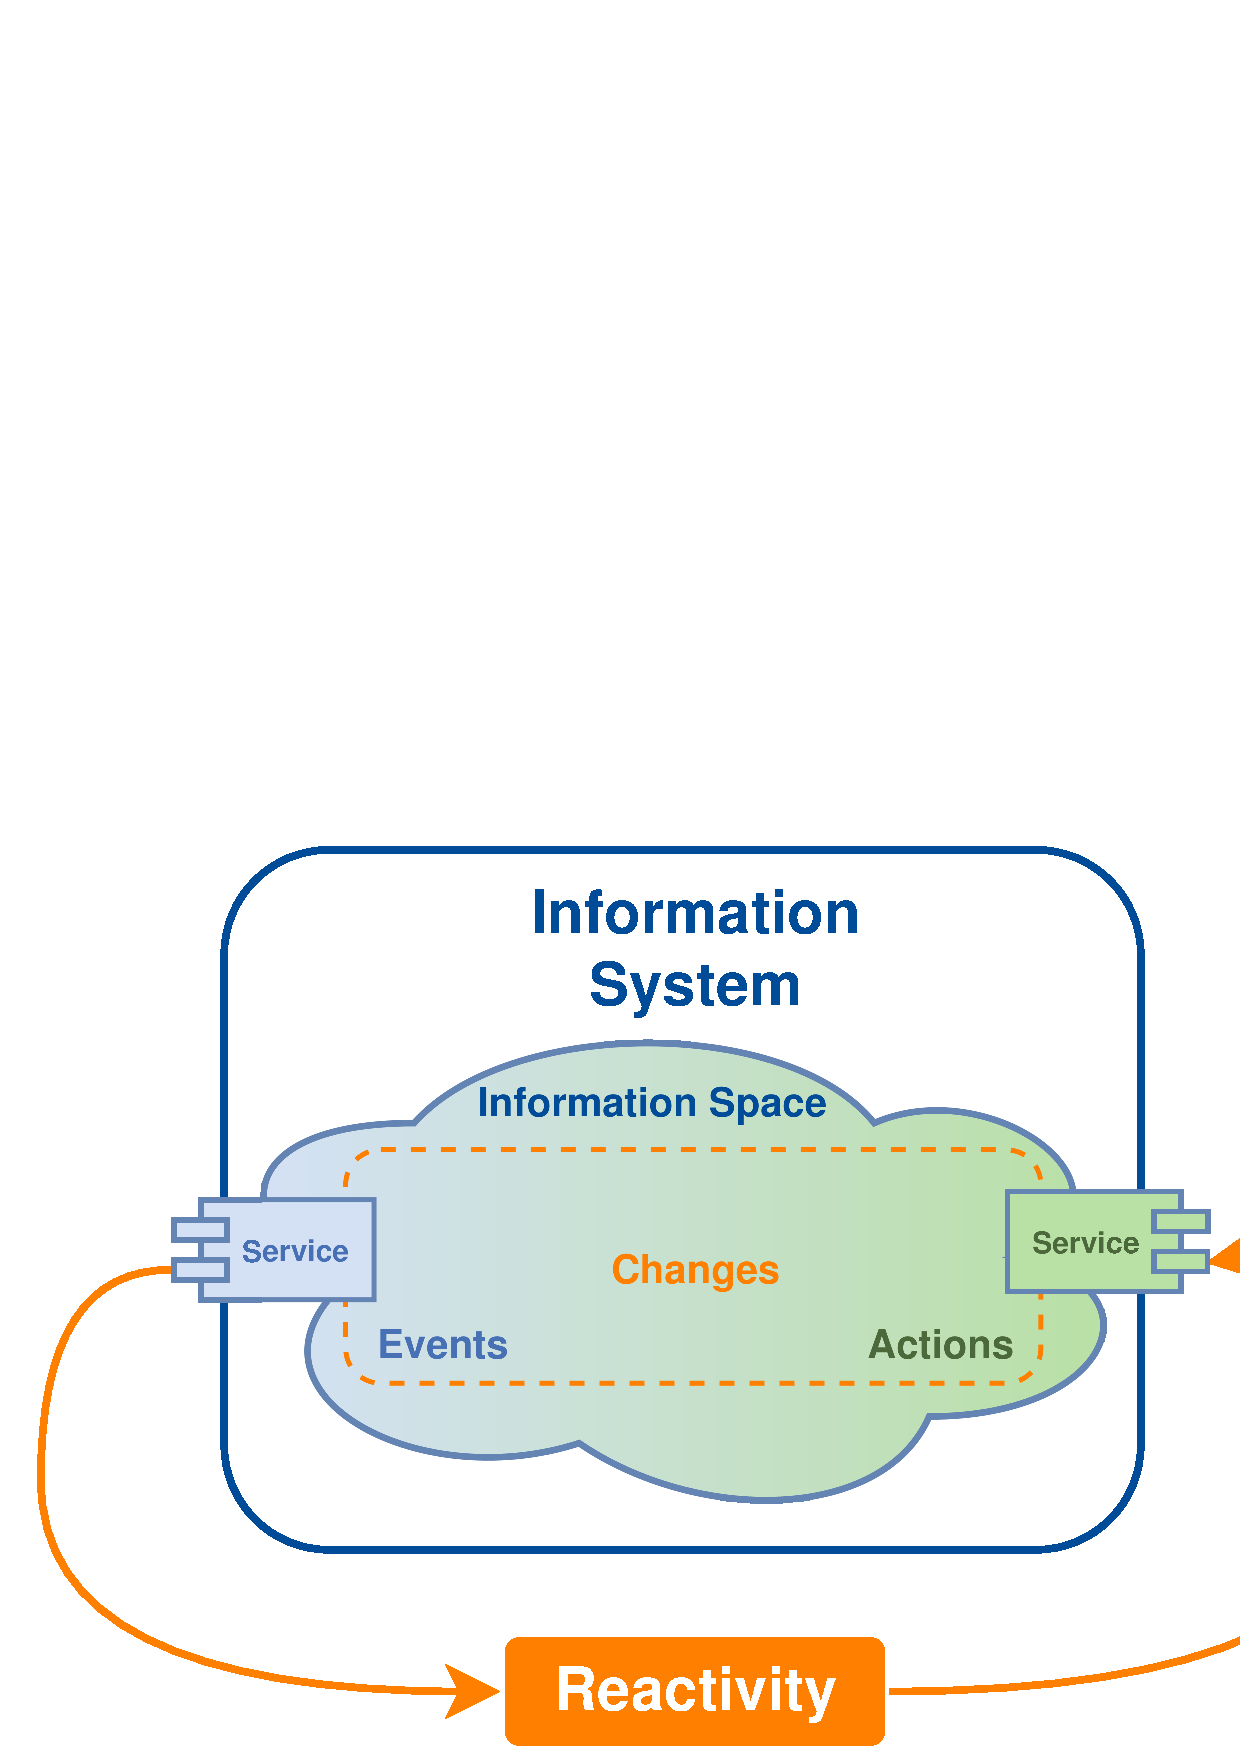
\includegraphics[width=0.7\textwidth]{figures/IS_InformationSpace}
  \caption{Reactivity imposed on \textrm{\glspl{infosystem}} and their \textrm{\glspl{infospace}} over Services}
  \label{fig:IS_InformationSpace}
\end{figure}
Data changes within an \textrm{\gls{infosystem}} can be detected and imposed from the outside, if apropriate interfaces to the services exist.
We model the detection of data changes as events, and the imposition of such changes as actions, as shown in Figure \ref{fig:IS_InformationSpace}.
Through this we are able to introduce an event-based model that is capable to detect events and react on behalf of them by executing actions on any \textrm{\gls{infospace}}.
A more precise distinction of the required modules for such a reactivity imposing entity is displayed in Figure \ref{fig:Standard-Model-Template}.
Each of these modules is introduced in this chapter.
\begin{figure}[!ht]
  \centering
  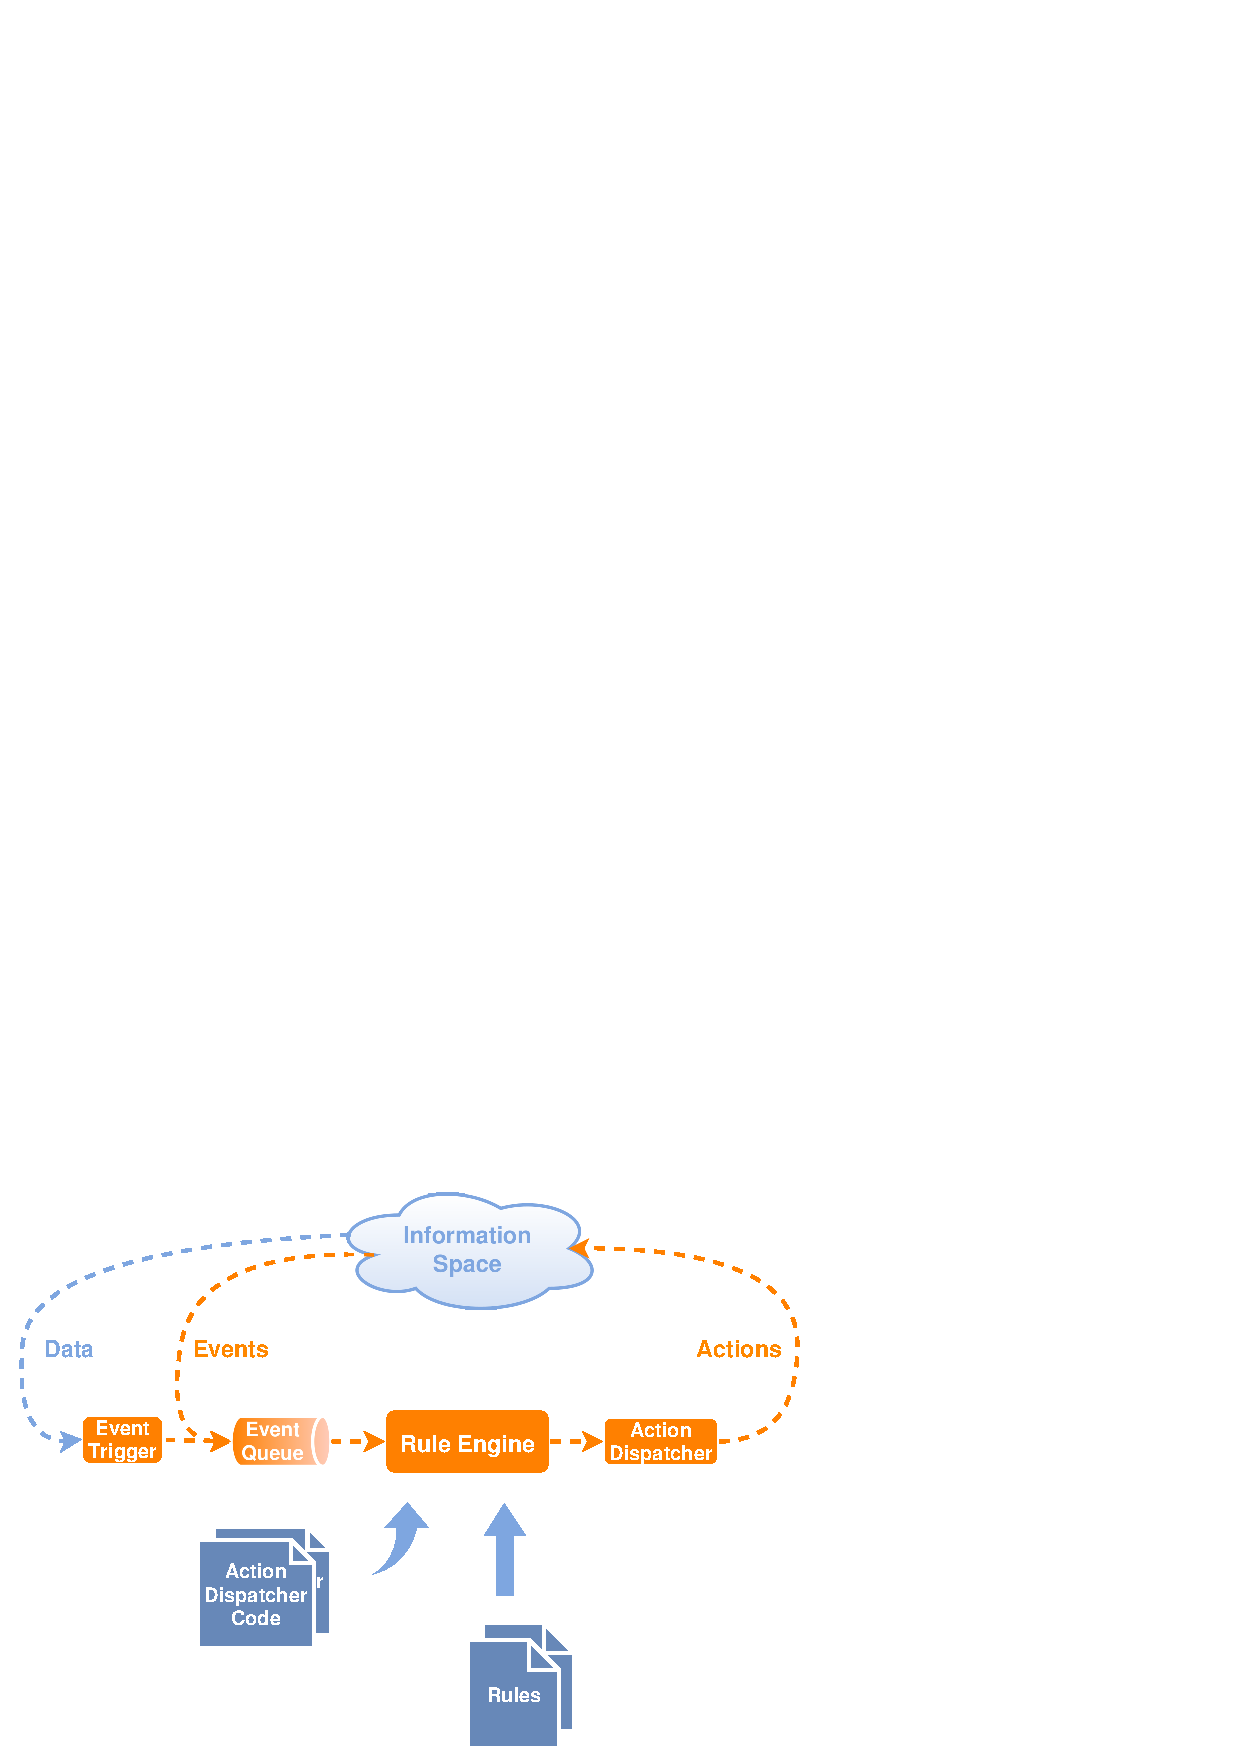
\includegraphics[width=0.8\textwidth]{figures/Standard-Model-Template}
  \caption{Conceptual Model for Reactive Information Systems and their Services}
  \label{fig:Standard-Model-Template}
\end{figure}



\section{From Physical Events to Virtual Events}
The \textrm{\gls{webofthings}}, where smart devices gain access to the Web, has already been mentioned shortly in the last chapter.
It is based on the \textrm{Internet of Things} which dealt with the incorporation of sensor networks into the Internet on the network level.
Such sensors bring the physical world directly into the virtual world.
This transformation pictures an important difference between physical and virtual events.
In physics, and in particular relativity, an event indicates a physical situation or occurrence, located at a specific point in space and time.
While physical events correspond to a physical situation which is located at a specific point in space and time, virtual events primarily consist of implicit parameters, i.e. a name and occurrence time.
These virtual events can be anywhere within \textrm{\glspl{infosystem}} at any point in time, thus their actual location differs most certainly from its occurrence.
Virtual events also have explicit parameters which correspond to available information about the event, such as the origin.
As soon as events are transformed into the virtual world, the afore mentioned location information is transformed into explicit event parameters.
But every virtual event has a name, an occurrence time and most likely some explicit parameters attached to it.
If the virtual event has a physical nature, it contains a physical location, if it has a virtual nature, it is likely associated with a virtual origin.
Since in our model events are changes in data of an \textrm{\gls{infospace}}, they can be virtually anything, e.g. physical measurements, changes on a static webpage, changes of the object behind a \textrm{\gls{webservice}} or a login attempt.



\section{Capturing Events from Information Systems}
The optimal case for an event-driven system which requires events from a remote \textrm{\gls{infosystem}} is, that events are triggered within the remote \textrm{\glspl{infosystem}} and then immediately communicated to interested parties, such as our envisioned reactivity imposing system.
Our research has shown that such \textrm{\glspl{infosystem}} are often passive and rarely provide ways for external systems to announce interest in changes of their data (e.g. in the context of \textrm{\glspl{webresource}}).
Many \textrm{\glspl{webresource}} provide access to their data over services, but do not actively communicate changes to interested parties.
This is where the upcoming concept of \textrm{\glspl{webhook}} comes into play.
Because of effectivity, it is essential for \textrm{\glspl{infosystem}} to push event notifications to external systems, instead of letting them poll for events.
Through them such pushed events it is possible to have real-time reactivity without high costs of continuously polling for changes over all \textrm{\glspl{infospace}}.
We also need to take passive \textrm{\glspl{infosystem}} into account which do not push events to external systems, therefore we need to incorporate polling for changes into our model.
Wherever an \textrm{\gls{infosystem}} is not capable to provide events to external \textrm{\glspl{infosystem}}, we can still read all the accessible data and detect changes in it, define them as events and feed them into our model.
In our model the polling for changes is incorporated in the \textrm{Event Trigger} modules.
Those are flexible modules have the proper tools to access any \textrm{\gls{infosystem}} service and therefore its \textrm{\gls{infospace}} and are capable of identifying changes in the data.
For example the \textrm{\gls{www}}, is an information universe of interlinked documents, that a user can browse through.
Through our model, we can pull changes in the data on the \textrm{\gls{www}}, i.e. document changes, and turn them into events.
These events which are derived from changes in the data of \textrm{\gls{infosystem}} are then fed into the \textrm{Event Listener}.
The \textrm{Event Listener} also pulls events directly from the \textrm{\glspl{infosystem}} that offers service functions which represent events but still need to be requested actively, e.g. new mail in inbox.



\section{Event Pattern Detection}
Traditional \textrm{\acrshort{eca}} systems only react on single events, but this might often not be enough to detect meaningful situations.
Primitive events occur at a point in time (e.g. a mouse button press event).
When they are composed (e.g. the latter event with a mouse release event), they turn into a composite event which is more complex and also has a duration.
Such a temporal event composition yields the chance to detect meaningful situations out of primitive events and react on them.
This is why there is a trend towards the detection of complex event patterns, as we have pointed out in the last chapter.
\textrm{\acrshort{cep}} could be incorporated into the rules of the \textrm{Rule Engine}, which then reacts on event patterns.
Though such an approach opposes our vision of a successively growing complexity of composite events, which are defined on top of each other and are fed back into the \textrm{Event Listener}.
Thus in our model an \textrm{Event Composition} module composes events into more complex events according to \textrm{\acrshort{ced}} definitions.
It is a very active research field, which has seen interesting studies\cite{akdere2008plan}\cite{2004_1265833} and outcomes\footnote{such as http://drools.jboss.org/drools-fusion.html} that could be incorporated into our model.
Such an event composing service systems works loosely coupled an could be realized by any suitable system, as described in \cite{robins2010complex}.



\section{Imposing Reactivity to Information Spaces}
In the last chapter we gave an introduction into reactivity and the \textrm{\acrshort{eca}} paradigm as an approach to achieve it.
So far in the introduction to our model we have introduced the foundation for an \textrm{\acrlong{eda}}.
We also need a module that translates events into actions on \textrm{\glspl{infosystem}}.
Almost all existing \textrm{\acrshort{eca}} system actions write on the local \textrm{\gls{infospace}} which opposes our vision of the orchestration of different \textrm{\glspl{infosystem}} in order to impose reactivity on top of or between them.
For that reason we introduce the \textrm{Action Dispatcher} modules which are located right behind the \textrm{Rule Engine} in terms of the data flow and complete the reactivity flow between heterogeneous \textrm{\glspl{infosystem}}.
\textrm{Action Dispatcher} modules are an important part of our model because they allow flexible coupling with \textrm{\gls{infosystem}} services, much like the \textrm{Event Trigger} modules do.
\textrm{Event Trigger} and \textrm{Action Dispatcher} modules are communication abstractions to services of \textrm{\glspl{infosystem}}, that allow us to deal with their heterogeneity in terms of communication.
The \textrm{\gls{infospace}} of an \textrm{\gls{infosystem}} is not limited to internal data, but can also reflect a coupling with other devices, and the sensing and controlling of it.
Thinking of the \textrm{\gls{webofthings}} this could include an \textrm{Action Dispatcher} that has access to an \textrm{\gls{infosystem}} which controls devices.
Through this it is, for example, capable of turning down the heating in a house, as shown in Figure \ref{fig:InformationSystemWoT}.
\begin{figure}[!ht]
  \centering
  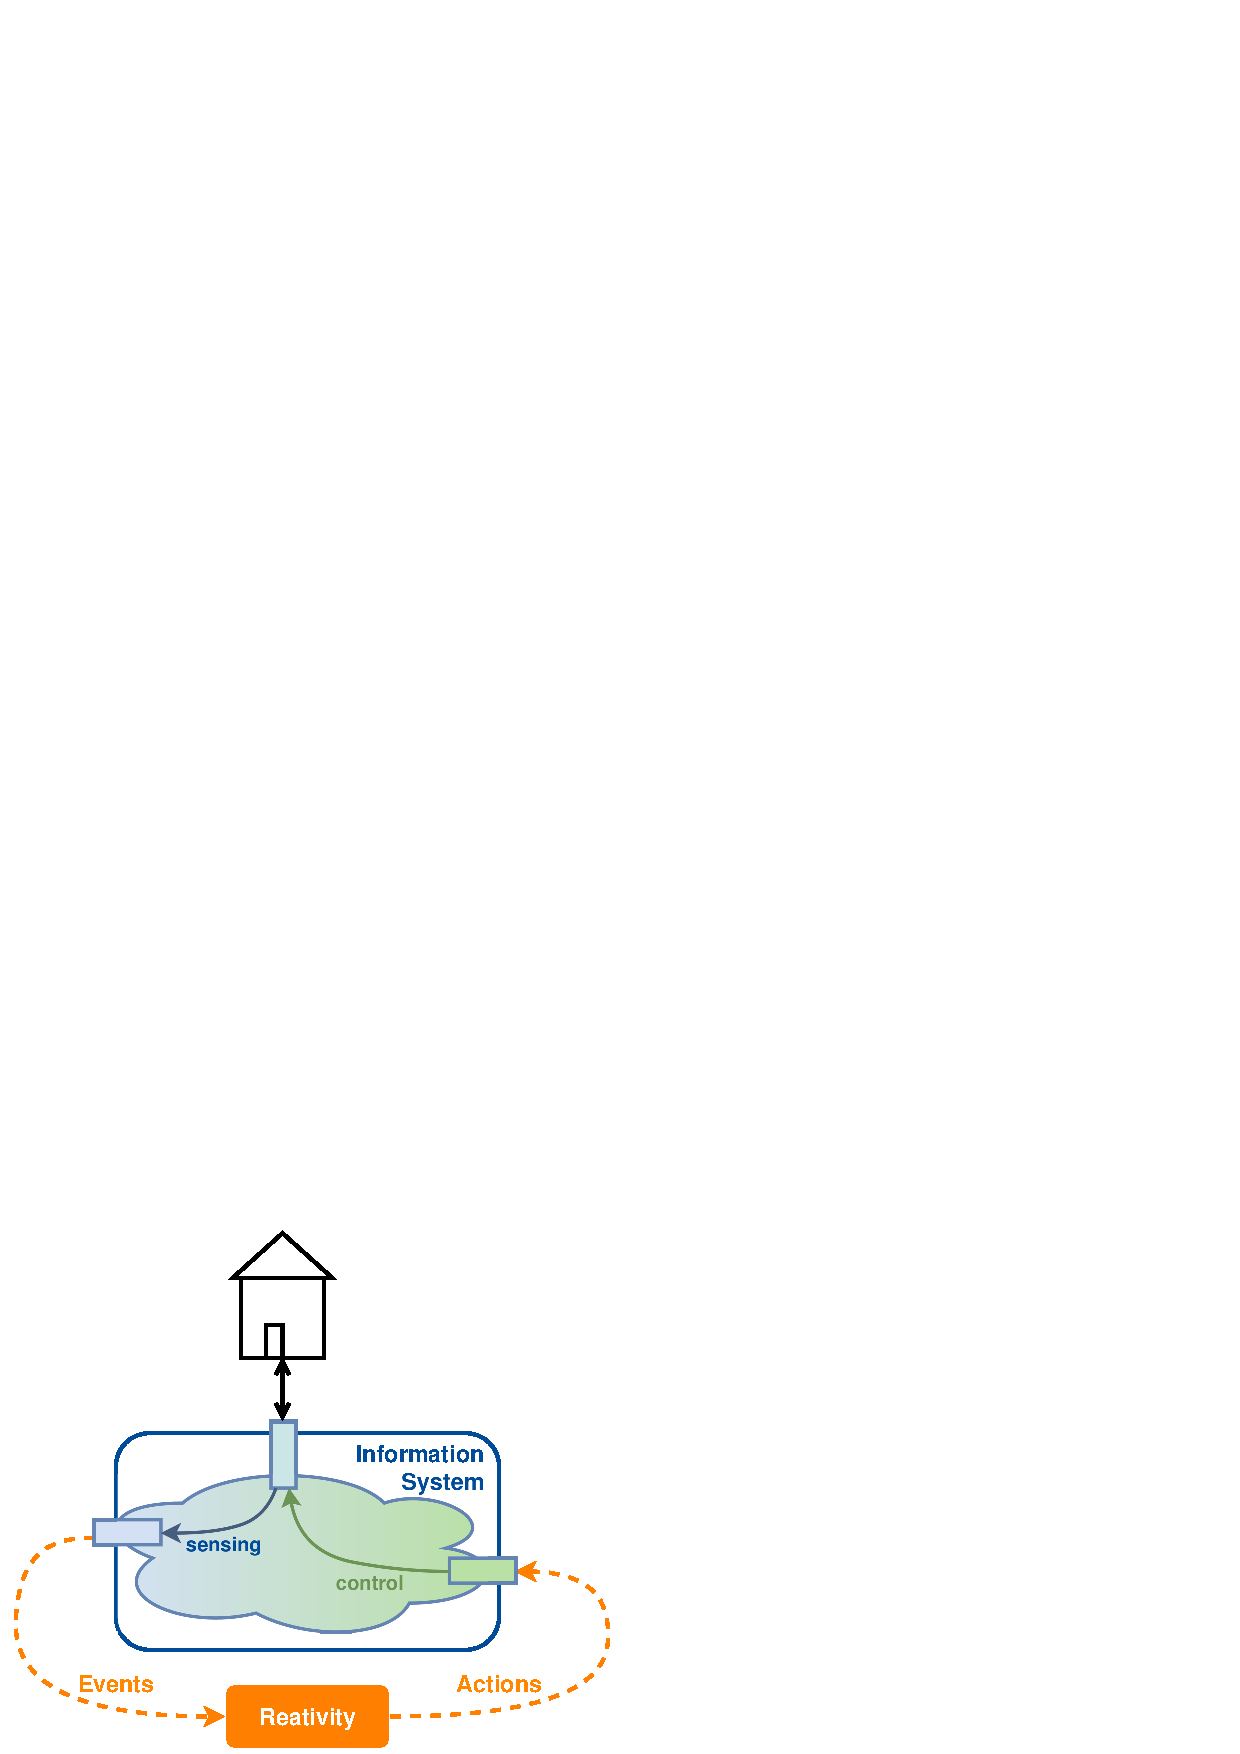
\includegraphics[width=0.6\textwidth]{figures/InformationSystemWoT}
  \caption{\textrm{\glspl{infosystem}} providing access to the \textrm{\gls{webofthings}} over their Services}
  \label{fig:InformationSystemWoT}
\end{figure}

So far we defined all the modules to access \textrm{\glspl{infosystem}} over their services, therefore we are able to define a \textrm{Rule Engine} that orchestrates them in a reactive way.
We have shown in the last chapter that \textrm{\acrshort{eca}} rules consist of three parts; an event to be recognized, conditions to be evaluated on the event and actions to be executed if an event triggers the rule through valid conditions.
In our model events are coming from the \textrm{Event Listener} to the \textrm{Rules Engine}, which checks all rules against the incoming event.
If any conditiong section of an active \textrm{\acrshort{eca}} rule evaluates to true, the action section (consisting of different \textrm{Action Dispatchers}) of that specific rule is executed.
Through this we described a complete reactive cycle that is able to impose reactivity on top of any existing \textrm{\gls{infosystem}}, if appropriate services exist.
